\documentclass[12pt]{article}
\usepackage[margin=1in]{geometry}
\usepackage{graphicx}
\usepackage{booktabs}
\usepackage{array}
\usepackage{hyperref}
\usepackage{tabularx}
\usepackage{fancyhdr}
\usepackage{color}
\usepackage{enumitem}
\usepackage{lastpage}

\hypersetup{
  colorlinks=true,
  linkcolor=blue,
  filecolor=blue,
  urlcolor=blue,
}

\setlength{\parindent}{0pt}
\pagestyle{fancy}
\fancyhf{}
\renewcommand{\headrulewidth}{0pt}

\fancyfoot[C]{Medical/Administrative Term Withdrawal Form - Page \thepage\ of \pageref{LastPage}}

\begin{document}

\begin{center}
  \textbf{\Large Medical/Administrative Term Withdrawal Request Form}\\[0.2cm]
  \textbf{Form ID: 2}\\[0.2cm]
  \textbf{Status: PENDING}
\end{center}

\hrule
\vspace{0.5cm}

\section*{1. Student Information}
\begin{tabular}{ll}
Name: & \textbf{jpgleite@CougarNet.UH.EDU d None} \\
myUH ID: & \textbf{d} \\
College: & \textbf{d} \\
Plan/Degree: & \textbf{d} \\
\end{tabular}

\vspace{0.5cm}

\section*{2. Current Mailing Address}
\begin{tabular}{ll}
Address: & \textbf{Noned} \\
City, State, Zip: & \textbf{d}, \textbf{d} \textbf{d} \\
Phone: & \textbf{None} \\
Email: & \textbf{jpgleite@CougarNet.UH.EDU} \\
\end{tabular}

\vspace{0.5cm}

\section*{3. Term Information}
\begin{tabular}{ll}
Term \& Year for Withdrawal: & \textbf{Fall 2024} \\
\end{tabular}

\vspace{0.5cm}

\section*{4. Last Date Attended Classes}
\begin{tabular}{ll}
Last Date: & \textbf{April 25, 2025} \\
\end{tabular}

\vspace{0.5cm}

\section*{5. Reason for Request}
\begin{tabular}{ll}
Type: & \textbf{Medical} \\
\end{tabular}

\noindent\textbf{Details:}\\
\fbox{\parbox{\dimexpr\textwidth-2\fboxsep-2\fboxrule}{
\vspace{0.2cm}
dd
\vspace{0.2cm}
}}

\vspace{0.5cm}

\section*{6. Additional Information}
\begin{tabular}{ll}
Financial Assistance: & \textbf{Yes} \\
UH Student Health Insurance: & \textbf{Yes} \\
Campus Housing: & \textbf{No} \\
F1/J1 Visa: & \textbf{No} \\
G.I. Bill Benefits: & \textbf{Yes} \\
\end{tabular}

\vspace{0.5cm}

\section*{7. Courses to be Withdrawn}
\begin{tabular}{lll}
\textbf{Subject} & \textbf{Number} & \textbf{Section} \\
\hline
33 & 333 & 33 \\

\end{tabular}

\vspace{0.5cm}

\section*{Acknowledgement}
\noindent\fbox{\parbox{\dimexpr\textwidth-2\fboxsep-2\fboxrule}{
I understand that a request for a medical or administrative term withdrawal is a request to withdraw from ALL courses I am/was enrolled in for the identified term. The request must be filed no later than 140 days following the close of the semester in which the coursework was taken. The withdrawal, when completed, does not entitle me to a refund if it occurs after State mandated refund periods (\textbf{3}, I understand). If I am eligible for a refund, it will be applied to any previous balance due, and if I received student financial assistance or a scholarship, I may be required to pay back all or a portion of it. In addition, I certify that the information I have provided is complete and true and I authorize the University to make any investigation of the facts in this request.
}}

\vspace{0.5cm}

\section*{Student Signature}
\begin{tabular}{ll}
Signature: & 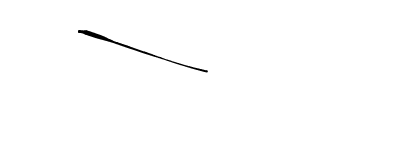
\includegraphics[width=5cm]{c:/Users/johnp/Desktop/Edmonton-v.02/static/temp/static/uploads/signatures/sig_1_20250424074627.png} \\
Date: & \textbf{April 24, 2025} \\
\end{tabular}

\vspace{0.5cm}

\section*{Request Information}
\begin{tabular}{ll}
Date Submitted: & \textbf{April 24, 2025} \\
Request Status: & \textbf{PENDING} \\
\end{tabular}



\label{LastPage}
\end{document}